% ============================================================
%  CHAPITRE III : Conception et réalisation
% ============================================================
\chapter{Conception et réalisation}
\label{chap:conception}

\section*{Introduction}

Ce chapitre détaille la démarche de conception de la plateforme, l'architecture retenue et les choix technologiques associés, la modélisation des données et de la méthodologie de scoring, ainsi que les principales étapes de réalisation, de test et de validation. Il présente également les résultats obtenus, les limites observées et les perspectives d'amélioration identifiées à l'issue du stage.

% -------------------------------------------------------
\section{Méthodologie et démarche}
\label{sec:methodologie}

\hspace{1cm}Le projet a été mené selon une démarche itérative en trois jalons, conforme au planning présenté au chapitre~\ref{chap:contexte} (section~\ref{sec:planification}). Chaque jalon a fait l'objet de points de contrôle hebdomadaires avec l'encadrant professionnel, le Dr.~Rachid Abouettahir, ainsi que d'un rapport de progression écrit en fin de jalon. Les trois rapports de progression produits (Jalon~1, Jalon~2, Jalon~3) documentent l'avancement jour par jour et ont été intégralement transmis et validés par l'encadrant.

% -------------------------------------------------------
\section{Architecture du système}
\label{sec:architecture}

\subsection{Vue d'ensemble}

La figure~\ref{fig:architecture} illustre l'architecture globale retenue pour le \gls{mvp} de la plateforme.

\begin{figure}[H]
  \centering
  \begin{tikzpicture}[
    node distance=1.2cm and 1.8cm,
    block/.style={
      rectangle, draw=iacsTeal, fill=iacsLight!50,
      rounded corners=5pt, minimum width=3.2cm,
      minimum height=1.2cm, align=center,
      font=\small\sffamily, line width=0.8pt,
      drop shadow={shadow xshift=1pt, shadow yshift=-1pt, opacity=0.1}
    },
    dbblock/.style={
      cylinder, draw=iacsTeal, fill=iacsGreen!15,
      shape border rotate=90, aspect=0.25,
      minimum width=2.2cm, minimum height=1.2cm,
      font=\small\sffamily, line width=0.8pt,
      align=center, cylinder uses custom fill,
      cylinder body fill=iacsGreen!15, cylinder end fill=iacsGreen!25
    },
    pdfblock/.style={
      block, fill=iacsOrange!15, draw=iacsOrange
    },
    arrow/.style={-Stealth, thick, color=iacsTeal},
    dataarrow/.style={-Stealth, thick, color=iacsAccent, dashed}
  ]
    % Couche interface
    \node[block] (ui) {\faDesktop\; Interface\\Streamlit};
    \node[block, right=of ui] (quest) {Questionnaire\\25 questions};
    \node[block, right=of quest] (score) {\textbf{Moteur de}\\\textbf{scoring}};

    % Couche données
    \node[dbblock, below=2.1cm of quest] (db) {SQLite\\7 tables};

    % Couche restitution
    \node[block, below=2.1cm of ui] (reco) {Recommandations\\priorisées};
    \node[pdfblock, below=2.1cm of score] (pdf) {\faFilePdf\; Export\\ReportLab};

    % Flèches
    \draw[arrow] (ui) -- (quest);
    \draw[arrow] (quest) -- (score);
    \draw[dataarrow] (quest) -- (db);
    \draw[dataarrow] (score) -- (db);
    \draw[arrow] (score) -- (pdf);
    \draw[arrow] (score) -- (reco);
    \draw[dataarrow] (reco) -- (pdf);

    % Labels couches
    \node[font=\footnotesize\sffamily\bfseries\color{iacsTeal},
          anchor=west] at ([xshift=-1cm, yshift=0.9cm]ui.north)
          {\faLayerGroup\; Couche interface};
    \node[font=\footnotesize\sffamily\bfseries\color{iacsGreen!60!black},
          anchor=west] at ([xshift=-1cm, yshift=1.6cm]db.north)
          {\faDatabase\; Couche données};
    \node[font=\footnotesize\sffamily\bfseries\color{iacsOrange},
          anchor=west] at ([xshift=-1cm, yshift=0.9cm]reco.north)
          {\faFile\; Couche restitution};
  \end{tikzpicture}
  \caption{Architecture globale de la plateforme d'auto-évaluation}
  \label{fig:architecture}
\end{figure}

\subsection{Stack technique retenue}

Le tableau~\ref{tab:technologies} résume les technologies et outils retenus pour le développement du \gls{mvp}.

\begin{table}[H]
  \centering
  \caption{Technologies et outils de développement}
  \label{tab:technologies}
  \renewcommand{\arraystretch}{1.4}
  \begin{tabularx}{\textwidth}{|>{\centering\arraybackslash}m{3.2cm}|l|X|}
    \hline
    \rowcolor{iacsTableHead}
    \textcolor{white}{\textbf{Catégorie}} &
    \textcolor{white}{\textbf{Outil}} &
    \textcolor{white}{\textbf{Rôle}} \\
    \hline
    Frontend/Backend & Streamlit (Python) & Framework unique pour le prototypage rapide de l'interface \\
    \hline
    \rowcolor{iacsLightGray}
    Base de données & SQLite & Persistance des \gls{pme}, audits, réponses et recommandations \\
    \hline
    Génération PDF & ReportLab~\cite{reportlab} & Génération du rapport de résultats exportable \\
    \hline
    \rowcolor{iacsLightGray}
    Authentification & bcrypt & Hachage des mots de passe (module développé, non intégré au flux principal) \\
    \hline
    Tests & pytest, \texttt{streamlit.testing.v1.AppTest} & Tests unitaires et tests de bout en bout sans navigateur \\
    \hline
  \end{tabularx}
\end{table}

\subsection{Justification des choix technologiques}

\textbf{Streamlit plutôt que Django/Flask+React.} Le choix de Streamlit~\cite{streamlit} répond à un besoin de rapidité de prototypage pour un \gls{mvp} à interface relativement simple. Ce framework unique évite la séparation frontend/backend, ce qui réduit la complexité d'intégration et permet une boucle de développement courte, adaptée à un stage de sept semaines.

\textbf{SQLite plutôt que PostgreSQL.} SQLite ne nécessite aucune infrastructure serveur dédiée et se révèle suffisant pour le volume d'usage visé, chaque audit étant réalisé par un utilisateur unique. La migration vers PostgreSQL est documentée comme perspective d'évolution (voir section~\ref{sec:perspectives}).

\textbf{ReportLab pour l'export PDF.} ReportLab permet une génération de \gls{pdf} en Python pur, avec un contrôle fin de la mise en page (jauge vectorielle, graphique en barres, tableaux), sans dépendance à un service externe.

\subsection{Structure des fichiers}
\label{sec:structure_fichiers}

L'application suit une architecture monolithique simple, volontairement choisie pour un \gls{mvp} développé en sept semaines : un seul processus Streamlit sert l'interface et exécute la logique métier, avec une base SQLite locale. Les modules \texttt{scoring.py} et \texttt{questionnaire.py} sont volontairement indépendants de Streamlit (aucun \texttt{import streamlit}), ce qui permet de les tester unitairement en isolation totale, sans lancer l'application. L'arborescence du dépôt est la suivante :

\begin{lstlisting}[language=bash, caption={Structure des fichiers du dépôt}, label={lst:structure}, basicstyle=\ttfamily\footnotesize\color{iacsDark}, frame=l]
cmrpi-platform/
|-- app.py                    # Application Streamlit (point d'entree)
|-- requirements.txt          # Dependances d'execution
|-- requirements-dev.txt      # Dependances de developpement (tests, lint)
|-- setup.cfg                 # Configuration flake8
|-- .github/workflows/ci.yml  # Integration continue
|
|-- src/
|   |-- auth.py               # Authentification (bcrypt)
|   |-- database.py           # Acces SQLite (CRUD)
|   |-- scoring.py            # Moteur de calcul du score
|   |-- questionnaire.py      # Chargement et validation du questionnaire
|   |-- pdf_generator.py      # Generation du rapport PDF
|   |-- ui_components.py      # Systeme de design (CSS, SVG)
|   `-- test_profiles.py      # 3 profils fictifs de demonstration
|
|-- data/
|   |-- questions/            # questions_fr.json, questions_en.json, guidance.json
|   |-- recommendations/      # Recommendations_Database.xlsx
|   `-- schema.sql            # Schema de la base de donnees
|
|-- scripts/
|   `-- init_db.py            # Initialisation de app.db
|
|-- tests/                    # 52 tests (unitaires + bout en bout)
|
`-- docs/
    `-- Scoring_Rules_V1.md   # Methodologie de scoring detaillee
\end{lstlisting}

% -------------------------------------------------------
\section{Modélisation}
\label{sec:modelisation}

\subsection{Schéma de données}

Le modèle de données repose sur sept tables : \texttt{pme}, \texttt{domain}, \texttt{question}, \texttt{audit}, \texttt{audit\_response}, \texttt{recommendation} et \texttt{audit\_log}. Les relations principales sont les suivantes : une \gls{pme} peut réaliser plusieurs audits ; chaque audit comporte 25 réponses ; les 25 questions sont réparties en 5 domaines de 5 questions chacun ; chaque recommandation est rattachée à un domaine et caractérisée par une sévérité (\textit{Critical}, \textit{High}, \textit{Medium}, \textit{Low}). La figure~\ref{fig:er} présente le diagramme entité-association simplifié.

\begin{figure}[H]
  \centering
  \begin{tikzpicture}[
    entity/.style={
      rectangle, draw=iacsTeal, fill=iacsLight!40,
      rounded corners=3pt, minimum width=2.6cm,
      minimum height=0.9cm, align=center,
      font=\small\sffamily\bfseries, line width=0.8pt
    },
    rel/.style={font=\scriptsize\sffamily\color{iacsGray}},
    arrow/.style={-Stealth, thick, color=iacsAccent}
  ]
    \node[entity] (pme) {pme};
    \node[entity, right=2.4cm of pme] (audit) {audit};
    \node[entity, right=2.4cm of audit] (response) {audit\_response};
    \node[entity, below=1.4cm of audit] (question) {question};
    \node[entity, left=2.4cm of question] (domain) {domain};
    \node[entity, right=2.4cm of question] (reco) {recommendation};
    \node[entity, below=1.4cm of pme] (log) {audit\_log};

    \draw[arrow] (pme) -- node[rel, above]{1..N} (audit);
    \draw[arrow] (audit) -- node[rel, above]{25} (response);
    \draw[arrow] (question) -- node[rel, right]{} (response);
    \draw[arrow] (domain) -- node[rel, above]{5} (question);
    \draw[arrow] (domain) -- (reco);
    \draw[arrow] (audit) -- (log);
  \end{tikzpicture}
  \caption{Diagramme entité-association simplifié du schéma de données}
  \label{fig:er}
\end{figure}

\subsection{Questionnaire}

Le questionnaire comprend 25 questions réparties sur les 5 domaines présentés au chapitre~\ref{chap:etat_art}, disponibles en français et en anglais avec un texte de guidance associé à chaque question. Le format retenu est une échelle de Likert à cinq niveaux, dont les libellés sont contextualisés à chaque question plutôt que numériques génériques. Le tableau~\ref{tab:likert} illustre ce principe pour une question relative à la politique de gouvernance.

\begin{table}[H]
  \centering
  \caption{Exemple d'échelle de Likert contextualisée (domaine Gouvernance)}
  \label{tab:likert}
  \renewcommand{\arraystretch}{1.3}
  \begin{tabularx}{\textwidth}{|c|X|}
    \hline
    \rowcolor{iacsTableHead}
    \textcolor{white}{\textbf{Niveau}} & \textcolor{white}{\textbf{Libellé}} \\
    \hline
    1 & Non \\
    \hline
    \rowcolor{iacsLightGray}
    2 & Partiellement \\
    \hline
    3 & Approuvée (1--2 ans) \\
    \hline
    \rowcolor{iacsLightGray}
    4 & Approuvée + revue annuelle \\
    \hline
    5 & Approuvée + revue + communiquée \\
    \hline
  \end{tabularx}
\end{table}

\subsection{Méthodologie de scoring}
\label{sec:scoring}

\hspace{1cm}La méthodologie de scoring constitue le c\oe{}ur méthodologique du projet. Le score d'un domaine est calculé à partir de la moyenne des réponses de Likert (1 à 5) obtenues pour les cinq questions de ce domaine, ramenée à une échelle de 0 à 100 selon l'équation~\eqref{eq:domain_score} :

\begin{equation}
  \text{Score}_{\text{domaine}} = \frac{\overline{\text{Likert}} - 1}{4} \times 100
  \label{eq:domain_score}
\end{equation}

où $\overline{\text{Likert}}$ désigne la moyenne des réponses du domaine sur l'échelle de 1 à 5. Le score global de la \gls{pme} est ensuite obtenu par la moyenne arithmétique des cinq scores de domaine, selon l'équation~\eqref{eq:global_score} :

\begin{equation}
  \text{Score}_{\text{global}} = \frac{1}{5}\sum_{i=1}^{5} \text{Score}_{\text{domaine}_i}
  \label{eq:global_score}
\end{equation}

Le score global obtenu est ensuite interprété selon quatre niveaux de maturité. Les seuils retenus, présentés au tableau~\ref{tab:seuils} sous forme d'intervalles semi-ouverts sans chevauchement de bornes, sont inspirés de la structuration en paliers du modèle \gls{cmmi}~\cite{humphrey1989} et correspondent exactement à la logique de comparaison stricte (\texttt{score < threshold}) implémentée dans la fonction \texttt{get\_maturity\_level()} du module \texttt{src/scoring.py}.

\begin{table}[H]
  \centering
  \caption{Seuils de maturité cybersécurité}
  \label{tab:seuils}
  \renewcommand{\arraystretch}{1.3}
  \begin{tabular}{|c|l|}
    \hline
    \rowcolor{iacsTableHead}
    \textcolor{white}{\textbf{Plage de score}} & \textcolor{white}{\textbf{Niveau de maturité}} \\
    \hline
    $[0, 25[$ \,\% & Critique \\
    \hline
    \rowcolor{iacsLightGray}
    $[25, 50[$ \,\% & Faible \\
    \hline
    $[50, 75[$ \,\% & Moyen \\
    \hline
    \rowcolor{iacsLightGray}
    $[75, 100]$ \,\% & Avancé \\
    \hline
  \end{tabular}
\end{table}

\subsubsection{Logique de sélection des recommandations}

La sélection des recommandations a été affinée au cours du Jalon~3 afin de respecter précisément la consigne de l'encadrant : proposer deux à trois recommandations selon les réponses les plus faibles. L'algorithme~\ref{algo:reco} décrit cette logique, implémentée dans la fonction \texttt{generate\_top\_recommendations()} du module \texttt{src/scoring.py}.

\begin{algorithm}[H]
  \caption{Sélection des recommandations priorisées}
  \label{algo:reco}
  \KwEntree{Scores de domaine $\{S_1, \ldots, S_5\}$, catalogue de recommandations $\mathcal{R}$}
  \KwSortie{Liste priorisée de 2 à 3 recommandations}

  Trier les domaines par score croissant\;
  $\mathcal{L} \leftarrow \emptyset$\;
  \Pour{chaque domaine $d$, du plus faible au plus fort}{
    \uSi{$S_d < 60\,\%$}{
      Rechercher dans $\mathcal{R}$ les recommandations de sévérité \{Critical, High\} pour $d$\;
    }
    \Sinon{
      Rechercher dans $\mathcal{R}$ les recommandations de sévérité \{Medium, Low\} pour $d$\;
    }
    Ajouter les recommandations trouvées à $\mathcal{L}$\;
  }
  \Retour{les 2 à 3 premières recommandations de $\mathcal{L}$, domaines faibles priorisés}
\end{algorithm}

\subsubsection{Validation par profils de test}

La cohérence de la méthodologie de scoring a été vérifiée à l'aide de trois profils fictifs de \gls{pme}, dont les résultats sont résumés au tableau~\ref{tab:profils}.

\begin{table}[H]
  \centering
  \caption{Profils de test et scores obtenus}
  \label{tab:profils}
  \renewcommand{\arraystretch}{1.3}
  \begin{tabular}{|l|l|c|c|}
    \hline
    \rowcolor{iacsTableHead}
    \textcolor{white}{\textbf{Profil}} &
    \textcolor{white}{\textbf{Secteur}} &
    \textcolor{white}{\textbf{Score global}} &
    \textcolor{white}{\textbf{Niveau}} \\
    \hline
    PME Finance & Finance & 44,0\,\% & Faible \\
    \hline
    \rowcolor{iacsLightGray}
    PME Commerce & Commerce & 20,0\,\% & Critique \\
    \hline
    PME Technologie & Technologie & 83,0\,\% & Avancé \\
    \hline
  \end{tabular}
\end{table}

\iacsnote{Les premiers calculs manuels réalisés au Jalon~1 comportaient une erreur d'addition, qui a été corrigée et revérifiée automatiquement lors du codage du moteur de scoring au Jalon~2. Cet épisode illustre l'intérêt d'une validation croisée entre un calcul manuel initial et son implémentation automatisée, et a été traité comme un point de rigueur méthodologique plutôt qu'un simple correctif.}

\subsection{Diagrammes UML}

Huit diagrammes UML ont été produits au Jalon~1 (Mermaid.js) afin de formaliser la conception : diagramme de cas d'utilisation (3 acteurs, 9 cas d'utilisation), diagramme de séquence (audit \gls{pme}, benchmark administrateur), diagramme de classes (7 classes), diagramme d'activité, diagramme d'état (5 états d'un audit), diagramme de composants (4 tiers) et diagramme de déploiement. Seul le diagramme de cas d'utilisation est reproduit dans ce rapport, sous une forme simplifiée redessinée en TikZ (figure~\ref{fig:use_case}) ; les sept autres diagrammes ne sont pas reproduits ici et restent disponibles dans leur intégralité dans le rapport de progression du Jalon~1, sur le dossier Drive du projet.

\begin{figure}[H]
  \centering
  \begin{tikzpicture}[
    actor/.style={font=\small\sffamily},
    usecase/.style={
      ellipse, draw=iacsTeal, fill=iacsLight!30,
      minimum width=3cm, minimum height=1cm,
      font=\small\sffamily, align=center
    }
  ]
    % Acteurs
    \node[actor] (pme) at (0,0) {\faUserTie};
    \node[below=0.1cm of pme, font=\scriptsize\sffamily] {Dirigeant PME};

    \node[actor] (admin) at (0,-4) {\faUserShield};
    \node[below=0.1cm of admin, font=\scriptsize\sffamily] {Administrateur};

    % Cas d'utilisation
    \node[usecase] (audit) at (5, 0) {Réaliser un\\audit};
    \node[usecase] (result) at (5, -1.5) {Consulter les\\résultats};
    \node[usecase] (export) at (5, -3) {Exporter le\\rapport PDF};
    \node[usecase] (manage) at (5, -4.5) {Gérer le\\catalogue};

    % Relations
    \draw[iacsTeal] (pme) -- (audit);
    \draw[iacsTeal] (pme) -- (result);
    \draw[iacsTeal] (pme) -- (export);
    \draw[iacsTeal] (admin) -- (manage);
    \draw[iacsTeal, dashed] (admin) -- (result);

    % Système
    \draw[iacsTeal, rounded corners=8pt, thick]
      (3, 1) rectangle (7.5, -5.5);
    \node[font=\footnotesize\sffamily\bfseries\color{iacsTeal}]
      at (5.25, 0.7) {Plateforme d'auto-évaluation};
  \end{tikzpicture}
  \caption{Diagramme de cas d'utilisation (version simplifiée)}
  \label{fig:use_case}
\end{figure}

% -------------------------------------------------------
\section{Réalisation}
\label{sec:realisation}

\subsection{Interface applicative}

L'interface développée sous Streamlit comprend trois écrans principaux : l'accueil (avec sélection du mode d'affichage), le questionnaire et les résultats.

\iacsnote{Le cahier des charges de l'encadrant spécifiait \enquote{une question par écran \textbf{ou} par section}. Plutôt que de n'implémenter qu'une seule de ces deux options, un sélecteur a été ajouté afin de proposer les deux modes au choix de l'utilisateur : cinq écrans de cinq questions chacun, ou vingt-cinq écrans d'une question chacun. Ce choix illustre une lecture attentive du cahier des charges, en couvrant l'ensemble des options proposées plutôt qu'un sous-ensemble.}

Le système de design retenu s'appuie sur la palette de couleurs du \gls{cmrpi} (navy \texttt{\#14213D}, teal \texttt{\#0E7C7B}, sable \texttt{\#C9A46A}) et sur les typographies Space Grotesk, Inter et JetBrains Mono. Un graphique radar \gls{svg} sur mesure a été développé pour visualiser les cinq scores de domaine, ce choix étant jugé plus pertinent qu'un simple graphique en barres pour une évaluation structurée en cinq axes.

\begin{figure}[H]
  \centering
  \begin{subfigure}[b]{0.31\textwidth}
    \centering
    \fbox{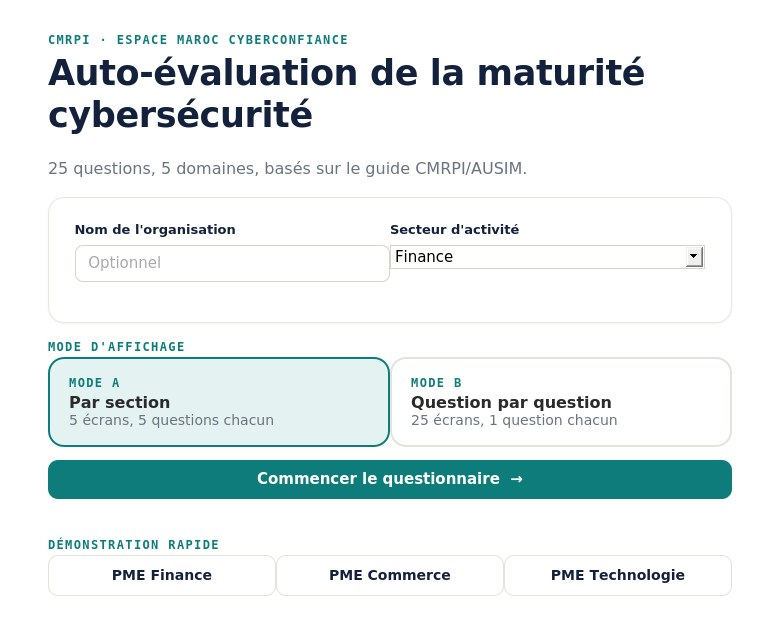
\includegraphics[width=\linewidth]{figures/01_accueil.jpg}}
    \caption{Accueil et sélection du mode}
    \label{fig:screen_home}
  \end{subfigure}
  \hfill
  \begin{subfigure}[b]{0.31\textwidth}
    \centering
    \fbox{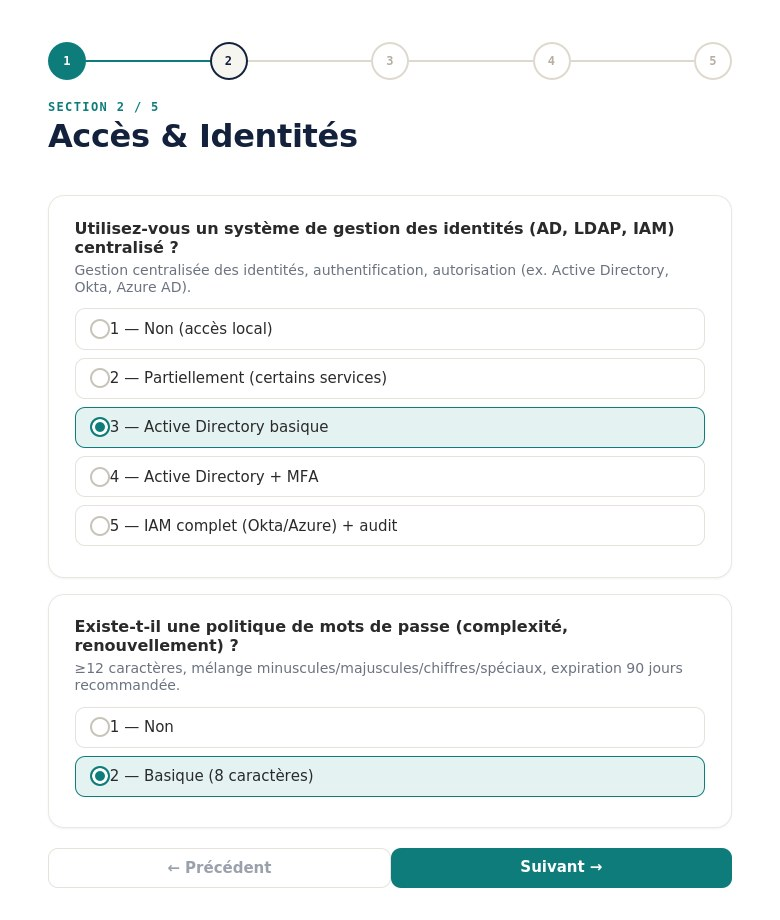
\includegraphics[width=\linewidth]{figures/02_questionnaire_section.jpg}}
    \caption{Questionnaire (mode section)}
    \label{fig:screen_questionnaire}
  \end{subfigure}
  \hfill
  \begin{subfigure}[b]{0.31\textwidth}
    \centering
    \fbox{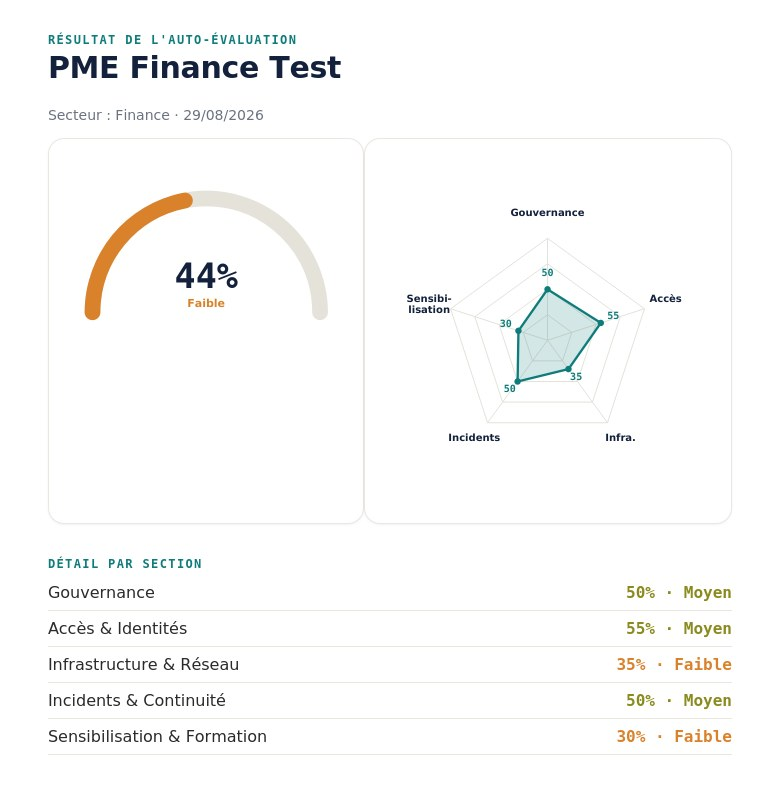
\includegraphics[width=\linewidth]{figures/03_resultats.jpg}}
    \caption{Résultats avec radar chart}
    \label{fig:screen_results}
  \end{subfigure}
  \caption{Captures d'écran des trois étapes du parcours utilisateur (profil \enquote{PME Finance Test})}
  \label{fig:screenshots}
\end{figure}

L'écran d'accueil (figure~\ref{fig:screen_home}) permet de renseigner facultativement le nom de l'organisation et son secteur, de choisir le mode d'affichage du questionnaire, et de charger instantanément un profil de démonstration. L'écran de questionnaire (figure~\ref{fig:screen_questionnaire}) illustre le mode \enquote{section}, ici pour le domaine Accès~\&~Identités : chaque question affiche son texte, un texte de guidance contextualisé et cinq options de réponse sous forme de cartes sélectionnables, avec un indicateur en pastilles matérialisant la progression à travers les cinq domaines. L'écran de résultats (figure~\ref{fig:screen_results}) affiche la jauge de score global colorée selon le niveau de maturité, le radar chart des cinq scores de domaine, ainsi que le détail par domaine. Dans les deux modes de questionnaire, le bouton \enquote{Suivant} reste désactivé tant que la section ou la question en cours n'a pas de réponse.

\subsection{Export PDF}

Le rapport de résultats généré par ReportLab (figure~\ref{fig:pdf_export}) comprend un en-tête aux couleurs du \gls{cmrpi}, un tableau d'identification de la \gls{pme}, une jauge en arc colorée selon le niveau de maturité obtenu, un graphique en barres des cinq scores de domaine, un tableau détaillé des réponses et deux à trois recommandations prioritaires accompagnées d'un badge de sévérité coloré (Critique, Haute, Moyenne, Basse).

\begin{figure}[H]
  \centering
  \begin{subfigure}[b]{0.47\textwidth}
    \centering
    \fbox{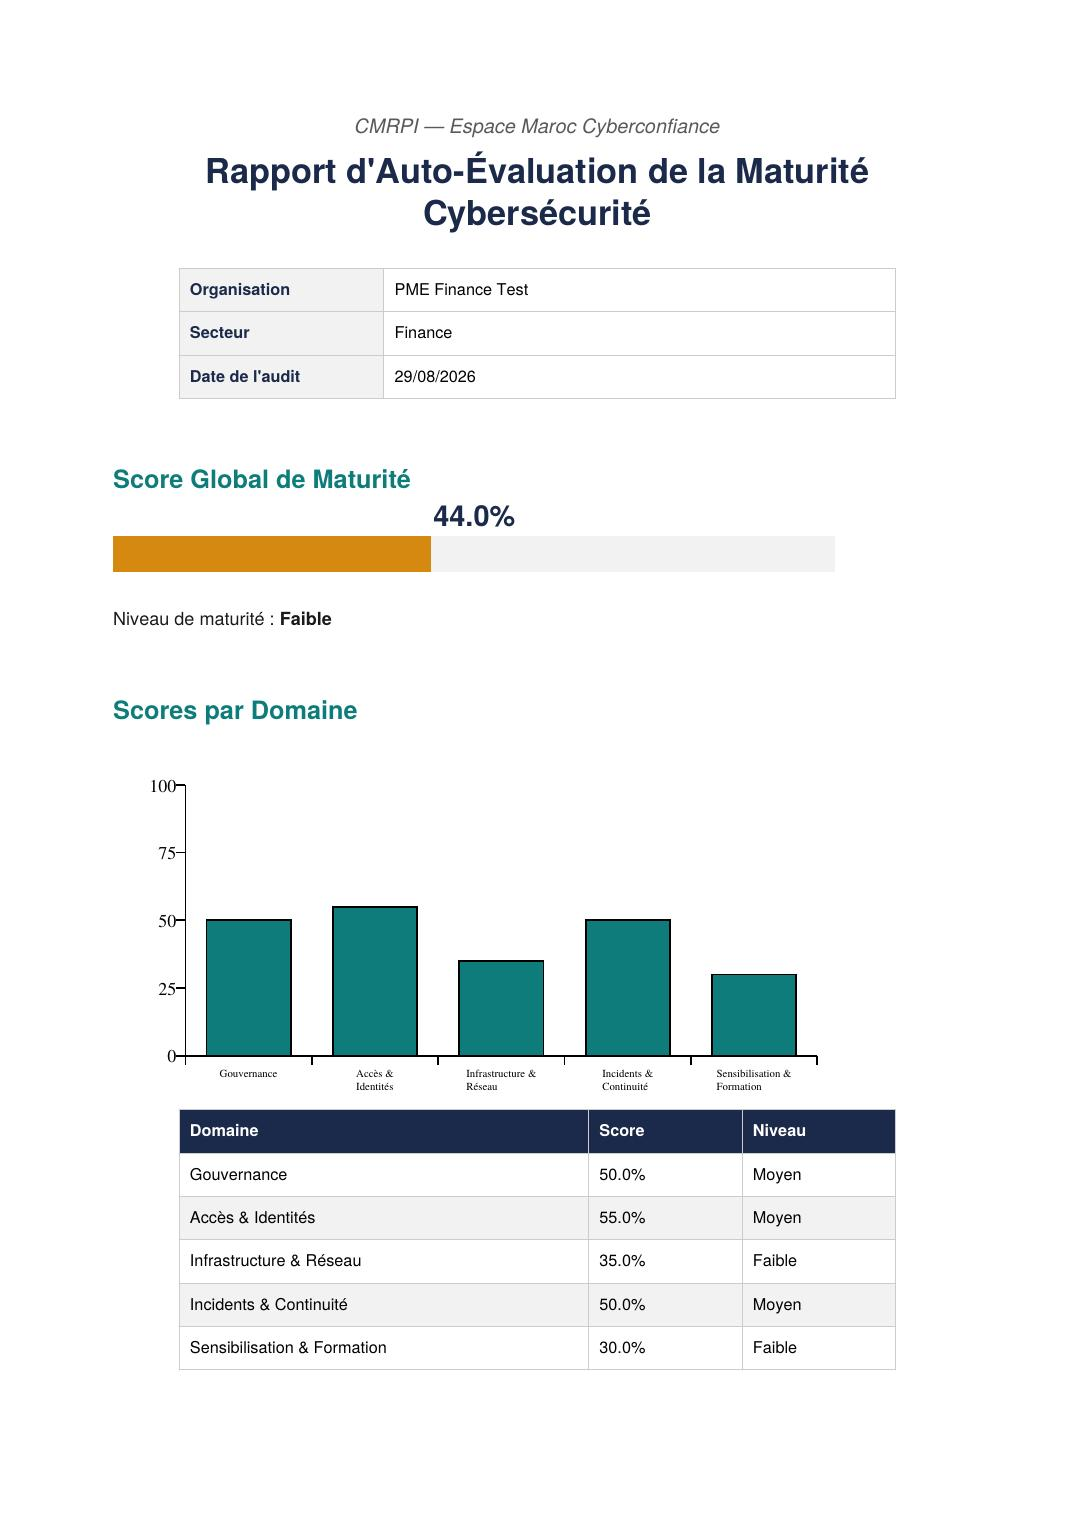
\includegraphics[width=\linewidth]{figures/pdf_page1.jpg}}
    \caption{Page 1 -- score global et scores par domaine}
    \label{fig:pdf_page1}
  \end{subfigure}
  \hfill
  \begin{subfigure}[b]{0.47\textwidth}
    \centering
    \fbox{
\includegraphics[width=\linewidth]{figures/pdf_page2.jpg}}
    \caption{Page 2 -- recommandations prioritaires}
    \label{fig:pdf_page2}
  \end{subfigure}
  \caption{Rapport PDF exporté (profil \enquote{PME Finance Test}, score global 44,0\,\%)}
  \label{fig:pdf_export}
\end{figure}

\subsection{Profils fictifs de test intégrés}

Conformément à l'exigence du brief du Jalon~2 (\enquote{tester avec 2--3 profils fictifs de \gls{pme}}), les trois profils présentés au tableau~\ref{tab:profils} peuvent être chargés en un clic depuis l'écran d'accueil, via le module \texttt{src/test\_profiles.py}, afin de faciliter les démonstrations rapides de la plateforme.

% -------------------------------------------------------
\section{Référence des modules}
\label{sec:modules}

\hspace{1cm}Cette section documente les fonctions publiques des principaux modules du dossier \texttt{src/}, à des fins de maintenabilité et de reprise du projet par un futur développeur.

\subsection{\texttt{scoring.py} -- moteur de calcul du score}

Module Python pur, sans aucune dépendance externe (ni Streamlit, ni base de données), ce qui permet de le tester et de le réutiliser indépendamment de l'interface. Le tableau~\ref{tab:mod_scoring} recense l'intégralité des neuf fonctions publiques du module, telles qu'elles figurent dans le fichier \texttt{src/scoring.py} du dépôt public à la date de rédaction de ce rapport.

\begin{longtable}{|>{\ttfamily\raggedright\scriptsize}p{4.8cm}|p{9.2cm}|}
  \caption{Fonctions publiques de \texttt{scoring.py} (dépôt public)} \label{tab:mod_scoring} \\
  \hline
  \rowcolor{iacsTableHead}
  \textcolor{white}{\textnormal{\textbf{Fonction}}} & \textcolor{white}{\textbf{Rôle}} \\
  \hline
  \endfirsthead
  \multicolumn{2}{c}{\tablename\ \thetable\ -- suite de la page précédente} \\
  \hline
  \rowcolor{iacsTableHead}
  \textcolor{white}{\textnormal{\textbf{Fonction}}} & \textcolor{white}{\textbf{Rôle}} \\
  \hline
  \endhead
  \hline
  \multicolumn{2}{r}{\textit{suite page suivante}} \\
  \endfoot
  \hline
  \endlastfoot
  calculate\_\allowbreak domain\_\allowbreak score(responses) & Calcule le score (0--100) d'un domaine à partir de ses 5 réponses Likert \\
  \hline
  \rowcolor{iacsLightGray}
  calculate\_\allowbreak domain\_\allowbreak scores(\allowbreak responses\_by\_domain) & Applique \texttt{\scriptsize calculate\_domain\_score} à chacun des domaines d'un dictionnaire \{domaine : réponses\} \\
  \hline
  calculate\_\allowbreak global\_\allowbreak score(domain\_scores) & Moyenne des scores de domaine, arrondie à une décimale \\
  \hline
  \rowcolor{iacsLightGray}
  get\_\allowbreak maturity\_\allowbreak level(score) & Retourne le niveau (Critique/Faible/Moyen/Avancé) selon le score \\
  \hline
  get\_\allowbreak severity\_\allowbreak filter(\allowbreak domain\_score) & Retourne le couple (sévérités à interroger, nombre maximal de recommandations) selon le score du domaine (seuil à 60\,\%) \\
  \hline
  \rowcolor{iacsLightGray}
  generate\_\allowbreak recommendations(\allowbreak domain\_scores,\allowbreak\ get\_recs\_fn) & Sélectionne, pour chaque domaine, les recommandations filtrées par sévérité et limitées par \texttt{\scriptsize get\_severity\_filter} -- version initiale (Jalon~2), conservée dans le module \\
  \hline
  generate\_\allowbreak top\_\allowbreak recommendations(\allowbreak domain\_scores,\allowbreak\ get\_recs\_fn,\allowbreak\ limit) & Sélectionne 2 à 3 recommandations globales priorisées, domaines les plus faibles en premier -- correctif du Jalon~3 (voir section~\ref{sec:scoring}) \\
  \hline
  score\_\allowbreak full\_\allowbreak audit(all\_responses) & Fonction principale : calcule scores de domaine, score global et niveau de maturité en un seul appel \\
  \hline
  \rowcolor{iacsLightGray}
  group\_\allowbreak responses\_\allowbreak by\_\allowbreak domain(\allowbreak responses,\allowbreak\ question\_domain\_map) & Regroupe les réponses brutes \{question\_id : valeur\} par domaine à partir de la correspondance question~$\rightarrow$~domaine \\
  \hline
\end{longtable}

\subsection{\texttt{database.py} -- accès aux données}

Toutes les fonctions de ce module utilisent un gestionnaire de contexte \texttt{get\_connection()} qui active les clés étrangères SQLite et valide automatiquement (\textit{commit}) les transactions. Le tableau~\ref{tab:mod_database} en présente les fonctions les plus significatives.

\begin{table}[H]
  \centering
  \caption{Fonctions principales de \texttt{database.py}}
  \label{tab:mod_database}
  \renewcommand{\arraystretch}{1.3}
  \small
  \begin{tabularx}{\textwidth}{|l|X|}
    \hline
    \rowcolor{iacsTableHead}
    \textcolor{white}{\textbf{Fonction}} & \textcolor{white}{\textbf{Rôle}} \\
    \hline
    \texttt{init\_database()} & Applique \texttt{data/schema.sql} (création des tables et amorçage des 5 domaines) \\
    \hline
    \rowcolor{iacsLightGray}
    \texttt{seed\_questions\_and\_domains(...)} & Charge les 25 questions depuis les fichiers JSON (idempotent) \\
    \hline
    \texttt{seed\_recommendations\_from\_xlsx(xlsx\_path)} & Charge les recommandations depuis le classeur Excel \\
    \hline
    \rowcolor{iacsLightGray}
    \texttt{create\_audit(pme\_id)} / \texttt{complete\_audit(...)} & Création d'un audit et clôture avec son score final \\
    \hline
    \texttt{save\_response(...)} & Enregistre une réponse individuelle à une question \\
    \hline
    \rowcolor{iacsLightGray}
    \texttt{get\_audit\_history(pme\_id)} & Historique des audits réalisés par une \gls{pme} \\
    \hline
    \texttt{log\_action(pme\_id, action, details)} & Journalisation d'une action dans \texttt{audit\_log} \\
    \hline
  \end{tabularx}
\end{table}

\subsection{Autres modules}

Le module \texttt{auth.py} fournit le hachage et la vérification bcrypt des mots de passe, ainsi que l'inscription et l'authentification d'une \gls{pme} ; il est fonctionnel et testé, mais n'est pas branché au flux principal de l'application, l'accès direct au questionnaire sans connexion ayant été retenu pour une expérience \enquote{simple à utiliser} conforme au brief du Jalon~2. Le module \texttt{questionnaire.py} charge les 25 questions et leur guidance depuis les fichiers JSON, et expose les regroupements par domaine utilisés par le mode \enquote{section}. Le module \texttt{pdf\_generator.py} construit le rapport \gls{pdf} via sa fonction principale \texttt{generate\_\allowbreak audit\_\allowbreak report(...)}, qui reçoit désormais une liste plate de recommandations plutôt qu'un dictionnaire par domaine, conformément à \texttt{scoring.\allowbreak generate\_\allowbreak top\_\allowbreak recommendations()}. Le module \texttt{ui\_components.py} centralise le système de design (feuille de style CSS, sélecteur de mode, indicateur de progression, génération du radar chart et de la jauge en \gls{svg}). Enfin, \texttt{test\_profiles.py} définit les trois profils fictifs de démonstration et leur conversion en réponses individuelles.

% -------------------------------------------------------
\section{Tests et validation}
\label{sec:tests}

\hspace{1cm}La qualité logicielle de la plateforme a été validée par une suite de 52 tests automatisés, atteignant 90\,\% de couverture de code (mesurée avec pytest-cov). Ces tests couvrent le moteur de scoring, l'authentification, la base de données, la génération \gls{pdf} et le questionnaire. Le tableau~\ref{tab:tests} détaille leur répartition par fichier.

\begin{table}[H]
  \centering
  \caption{Répartition de la suite de tests}
  \label{tab:tests}
  \renewcommand{\arraystretch}{1.3}
  \small
  \begin{tabularx}{\textwidth}{|l|c|X|}
    \hline
    \rowcolor{iacsTableHead}
    \textcolor{white}{\textbf{Fichier}} &
    \textcolor{white}{\textbf{Tests}} &
    \textcolor{white}{\textbf{Contenu}} \\
    \hline
    \texttt{test\_scoring.py} & 15 & Formules de score, seuils de maturité, sélection de recommandations \\
    \hline
    \rowcolor{iacsLightGray}
    \texttt{test\_questionnaire.py} & 8 & Chargement JSON, validation des réponses \\
    \hline
    \texttt{test\_profiles.py} & 3 & Cohérence des 3 profils de démonstration \\
    \hline
    \rowcolor{iacsLightGray}
    \texttt{test\_auth.py} & 8 & Inscription, connexion, hachage des mots de passe \\
    \hline
    \texttt{test\_database\_pdf.py} & 6 & CRUD base de données, génération \gls{pdf} \\
    \hline
    \rowcolor{iacsLightGray}
    \texttt{test\_app\_flow.py} & 12 & Tests de bout en bout (\texttt{AppTest}) : parcours complet, 2 modes, export \gls{pdf} \\
    \hline
    \textbf{Total} & \textbf{52} & \\
    \hline
  \end{tabularx}
\end{table}

Les tests de bout en bout utilisent \texttt{streamlit.testing.v1.AppTest}, le framework officiel Streamlit qui simule un utilisateur réel cliquant dans l'application, sans navigateur ni serveur à lancer manuellement. Ils couvrent notamment le chargement de l'accueil sans erreur, les trois profils de démonstration affichant le score exact attendu, la désactivation du bouton \enquote{Suivant} tant qu'une réponse manque, le parcours complet dans les deux modes jusqu'à l'écran de score, et la présence du bouton de téléchargement \gls{pdf} en fin de parcours.

Le code respecte par ailleurs les règles de style PEP~8, avec zéro erreur relevée par flake8 (longueur de ligne maximale fixée à 120 caractères dans \texttt{setup.cfg}). Un pipeline d'intégration continue (\texttt{.github/workflows/ci.yml}) exécute automatiquement, à chaque \textit{push} ou \textit{pull request}, l'installation des dépendances, la vérification flake8 sur \texttt{src/}, \texttt{app.py} et \texttt{tests/}, ainsi que l'ensemble de la suite pytest avec couverture, sur un environnement Python~3.12 entièrement vierge.

\iacswarning{Une vérification d'installation sur environnement vierge a révélé, au Jalon~3, trois régressions de dépendances : la bibliothèque \texttt{pandas}, non utilisée dans le code mais cassant l'installation sur Python~3.12 ; une version de \texttt{streamlit} trop ancienne, cassant les tests \texttt{AppTest} ; et une version de \texttt{flake8} trop ancienne générant de faux positifs sur les f-strings. Ces trois régressions ont été corrigées, revérifiées de bout en bout, et sont désormais prévenues par le pipeline d'intégration continue.}

% -------------------------------------------------------
\section{Fonctionnalités au-delà du périmètre strict}
\label{sec:bonus}

Deux fonctionnalités ont été développées au-delà du périmètre strict initialement défini : un module d'authentification par hachage bcrypt avec persistance multi-audits (historique des évaluations d'une même \gls{pme}), et l'export \gls{pdf}, qui est devenu périmètre officiel dès le Jalon~3. Ces éléments illustrent une anticipation des besoins au-delà du cahier des charges initial ; il convient toutefois de préciser que le module d'authentification n'est, à ce stade, pas pleinement intégré au flux principal validé.

% -------------------------------------------------------
\section{Résultats obtenus}
\label{sec:resultats}

Au terme du stage, la plateforme constitue un système fonctionnel de bout en bout, couvrant le parcours complet questionnaire~$\rightarrow$~score~$\rightarrow$~export \gls{pdf}. Elle a été validée par l'encadrant professionnel à chaque jalon, avec des retours explicites (\enquote{bravo, un livrable de qualité} au Jalon~1, \enquote{merci pour les résultats} au Jalon~2). Le code source est public et documenté à l'adresse \url{https://github.com/YOUSSEFKARROUM/PFA_CRMPI}, accompagné d'une documentation technique dédiée couvrant l'architecture, le guide d'installation, la référence des modules et le dépannage. Sur le plan de la qualité logicielle, le projet compte 52 tests automatisés, 90\,\% de couverture de code, un pipeline \gls{ci} opérationnel et une dette technique de lint nulle.

% -------------------------------------------------------
\section{Limites observées}
\label{sec:limites}

Plusieurs limites ont été identifiées à l'issue du stage :

\begin{itemize}
  \item Le périmètre reste mono-utilisateur ; le support multi-tenant complet n'est pas implémenté en production.
  \item La base SQLite n'est pas adaptée à une montée en charge au-delà d'une cinquantaine d'utilisateurs concurrents ; une migration vers PostgreSQL est identifiée comme nécessaire pour un passage en production.
  \item Le benchmarking anonymisé inter-\gls{pme} n'est pas encore implémenté.
  \item La plateforme n'est aujourd'hui exécutée qu'en local ; le déploiement en ligne reste à réaliser (voir ci-dessous).
\end{itemize}

% -------------------------------------------------------
\section{Perspectives d'amélioration}
\label{sec:perspectives}

Plusieurs pistes d'évolution ont été identifiées, certaines en concertation avec l'encadrant.

\textbf{Déploiement en ligne.} La procédure prévue -- non encore réalisée au moment de la rédaction de ce rapport -- consiste à déployer la plateforme sur Streamlit Community Cloud, l'option la plus rapide pour donner un accès en ligne à l'encadrant : création d'une application depuis le dépôt GitHub public (branche \texttt{main}, fichier \texttt{app.py}), installation automatique de \texttt{requirements.txt}, et initialisation automatique de la base au premier lancement si \texttt{app.db} n'existe pas encore. Un point de vigilance a toutefois été identifié : le système de fichiers de Streamlit Community Cloud n'est pas garanti persistant entre redéploiements, ce qui rend la migration vers une base hébergée (par exemple PostgreSQL managé) nécessaire au-delà d'un usage de démonstration.

\begin{enumerate}
  \item Migrer de Streamlit vers une architecture Django ou FastAPI côté serveur avec un frontend React, pour une version production multi-utilisateurs.
  \item Migrer la base de données de SQLite vers PostgreSQL, notamment pour garantir la persistance des données en déploiement cloud.
  \item Finaliser le déploiement sur Streamlit Community Cloud selon la procédure décrite ci-dessus.
  \item Mettre en place un benchmarking sectoriel anonymisé entre \gls{pme}.
  \item Étudier la faisabilité d'une certification \enquote{PME Cyber-Sûre}, piste évoquée avec l'encadrant.
  \item Étendre le questionnaire à des \textit{tracks} sectoriels spécialisés (Finance, Santé, E-commerce).
\end{enumerate}

\section*{Conclusion}

Ce chapitre a présenté la conception et la réalisation de la plateforme d'auto-évaluation de la maturité cybersécurité : architecture technique, modélisation des données et du questionnaire, méthodologie de scoring justifiée académiquement, réalisation de l'interface et de l'export \gls{pdf}, ainsi que les tests et résultats obtenus. Les limites observées et les perspectives identifiées tracent les prochaines étapes envisageables pour faire évoluer cette plateforme vers un usage en production.
